
\documentclass[%
oneside,                 % oneside: electronic viewing, twoside: printing
final,                   % draft: marks overfull hboxes, figures with paths
10pt]{article}

\listfiles               %  print all files needed to compile this document

\usepackage{relsize,makeidx,color,setspace,amsmath,amsfonts,amssymb}
\usepackage[table]{xcolor}
\usepackage{bm,ltablex,microtype}
\usepackage{markdown}
\usepackage{graphicx}

\usepackage[T1]{fontenc}
%\usepackage[latin1]{inputenc}
\usepackage{ucs}
\usepackage[utf8x]{inputenc}

\usepackage{lmodern}

% Hyperlinks in PDF:
\definecolor{linkcolor}{rgb}{0,0,0.4}
\usepackage{hyperref}
\hypersetup{
    breaklinks=true,
    colorlinks=true,
    linkcolor=linkcolor,
    urlcolor=linkcolor,
    citecolor=black,
    filecolor=black,
    %filecolor=blue,
    pdfmenubar=true,
    pdftoolbar=true,
    bookmarksdepth=3   % Uncomment (and tweak) for PDF bookmarks with more levels than the TOC
    }
%\hyperbaseurl{}   % hyperlinks are relative to this root

\setcounter{tocdepth}{2}  % levels in table of contents

% Tricks for having figures close to where they are defined:
% 1. define less restrictive rules for where to put figures
\setcounter{topnumber}{2}
\setcounter{bottomnumber}{2}
\setcounter{totalnumber}{4}
\renewcommand{\topfraction}{0.95}
\renewcommand{\bottomfraction}{0.95}
\renewcommand{\textfraction}{0}
\renewcommand{\floatpagefraction}{0.75}
% floatpagefraction must always be less than topfraction!
% 2. ensure all figures are flushed before next section
\usepackage[section]{placeins}
% 3. enable begin{figure}[H] (often leads to ugly pagebreaks)
%\usepackage{float}\restylefloat{figure}

\usepackage[framemethod=TikZ]{mdframed}

% --- begin definitions of admonition environments ---

% Admonition style "mdfbox" is an oval colored box based on mdframed
% "notice" admon
\colorlet{mdfbox_notice_background}{gray!5}
\newmdenv[
  skipabove=15pt,
  skipbelow=15pt,
  outerlinewidth=0,
  backgroundcolor=mdfbox_notice_background,
  linecolor=black,
  linewidth=2pt,       % frame thickness
  frametitlebackgroundcolor=mdfbox_notice_background,
  frametitlerule=true,
  frametitlefont=\normalfont\bfseries,
  shadow=false,        % frame shadow?
  shadowsize=11pt,
  leftmargin=0,
  rightmargin=0,
  roundcorner=5,
  needspace=0pt,
]{notice_mdfboxmdframed}

\newenvironment{notice_mdfboxadmon}[1][]{
\begin{notice_mdfboxmdframed}[frametitle=#1]
}
{
\end{notice_mdfboxmdframed}
}

% Admonition style "mdfbox" is an oval colored box based on mdframed
% "summary" admon
\colorlet{mdfbox_summary_background}{gray!5}
\newmdenv[
  skipabove=15pt,
  skipbelow=15pt,
  outerlinewidth=0,
  backgroundcolor=mdfbox_summary_background,
  linecolor=black,
  linewidth=2pt,       % frame thickness
  frametitlebackgroundcolor=mdfbox_summary_background,
  frametitlerule=true,
  frametitlefont=\normalfont\bfseries,
  shadow=false,        % frame shadow?
  shadowsize=11pt,
  leftmargin=0,
  rightmargin=0,
  roundcorner=5,
  needspace=0pt,
]{summary_mdfboxmdframed}

\newenvironment{summary_mdfboxadmon}[1][]{
\begin{summary_mdfboxmdframed}[frametitle=#1]
}
{
\end{summary_mdfboxmdframed}
}

% Admonition style "mdfbox" is an oval colored box based on mdframed
% "warning" admon
\colorlet{mdfbox_warning_background}{gray!5}
\newmdenv[
  skipabove=15pt,
  skipbelow=15pt,
  outerlinewidth=0,
  backgroundcolor=mdfbox_warning_background,
  linecolor=black,
  linewidth=2pt,       % frame thickness
  frametitlebackgroundcolor=mdfbox_warning_background,
  frametitlerule=true,
  frametitlefont=\normalfont\bfseries,
  shadow=false,        % frame shadow?
  shadowsize=11pt,
  leftmargin=0,
  rightmargin=0,
  roundcorner=5,
  needspace=0pt,
]{warning_mdfboxmdframed}

\newenvironment{warning_mdfboxadmon}[1][]{
\begin{warning_mdfboxmdframed}[frametitle=#1]
}
{
\end{warning_mdfboxmdframed}
}

% Admonition style "mdfbox" is an oval colored box based on mdframed
% "question" admon
\colorlet{mdfbox_question_background}{gray!5}
\newmdenv[
  skipabove=15pt,
  skipbelow=15pt,
  outerlinewidth=0,
  backgroundcolor=mdfbox_question_background,
  linecolor=black,
  linewidth=2pt,       % frame thickness
  frametitlebackgroundcolor=mdfbox_question_background,
  frametitlerule=true,
  frametitlefont=\normalfont\bfseries,
  shadow=false,        % frame shadow?
  shadowsize=11pt,
  leftmargin=0,
  rightmargin=0,
  roundcorner=5,
  needspace=0pt,
]{question_mdfboxmdframed}

\newenvironment{question_mdfboxadmon}[1][]{
\begin{question_mdfboxmdframed}[frametitle=#1]
}
{
\end{question_mdfboxmdframed}
}

% Admonition style "mdfbox" is an oval colored box based on mdframed
% "block" admon
\colorlet{mdfbox_block_background}{gray!5}
\newmdenv[
  skipabove=15pt,
  skipbelow=15pt,
  outerlinewidth=0,
  backgroundcolor=mdfbox_block_background,
  linecolor=black,
  linewidth=2pt,       % frame thickness
  frametitlebackgroundcolor=mdfbox_block_background,
  frametitlerule=true,
  frametitlefont=\normalfont\bfseries,
  shadow=false,        % frame shadow?
  shadowsize=11pt,
  leftmargin=0,
  rightmargin=0,
  roundcorner=5,
  needspace=0pt,
]{block_mdfboxmdframed}

\newenvironment{block_mdfboxadmon}[1][]{
\begin{block_mdfboxmdframed}[frametitle=#1]
}
{
\end{block_mdfboxmdframed}
}

% --- end of definitions of admonition environments ---

% prevent orhpans and widows
\clubpenalty = 10000
\widowpenalty = 10000

% --- end of standard preamble for documents ---


% insert custom LaTeX commands...

\raggedbottom
\makeindex
\usepackage[totoc]{idxlayout}   % for index in the toc
\usepackage[nottoc]{tocbibind}  % for references/bibliography in the toc

%-------------------- end preamble ----------------------

\begin{document}

% matching end for #ifdef PREAMBLE

\newcommand{\exercisesection}[1]{\subsection*{#1}}


% ------------------- main content ----------------------



% ----------------- title -------------------------

\thispagestyle{empty}

\begin{center}
{\LARGE\bf
\begin{spacing}{1.25}
Machine Learning and Artificial Intelligence in Nuclear Physics
\end{spacing}
}
\end{center}

% ----------------- author(s) -------------------------

\begin{center}
{\bf Daniel Bazin, Scott Bogner, Alexandra Gade, Yue Hao, Heiko Hergert, Morten Hjorth-Jensen, Dean Lee, Sean Liddick, Witek Nazarewicz, Filomena Nunes, Scott Pratt, Andrea Shindler, and Betty Tzang}
\end{center}

    \begin{center}
% List of all institutions:
{\small Department of Physics and Astronomy and Facility for Rare Ion Beams and National Superconducting Cyclotron Laboratory, Michigan State University, USA}
\end{center}
    
% ----------------- end author(s) -------------------------


\section{Machine Learning and AI in Nuclear Physics}


Artificial intelligence-based techniques, particularly in machine
learning and optimization, are increasingly being used in many areas
of experimental and theoretical physics to facilitate discovery,
accelerate data analysis and modeling efforts, and bridge different
physical and temporal scales in numerical models.

These techniques are proving to be powerful tools for advancing our
understanding; however, they are not without significant
challenges. The theoretical foundations of many tools, such as deep
learning, are poorly understood, resulting in the use of techniques
whose behavior (and misbehavior) is difficult to predict and
understand. Similarly, physicists typically use general AI techniques
that are not tailored to the needs of the experimental and theoretical
work being done. Thus, many opportunities exist for major advances
both in physical discovery using AI and in the theory of
AI. Furthermore, there are tremendous opportunities for these fields
to inform each other, for example, in creating machine learning- based
methods that must obey certain constraints by design, such as the
conservation of mass, momentum and energy.






\subsection{What is Machine Learning?}

Machine learning is the science of giving computers the ability to
learn without being explicitly programmed.  The idea is that there
exist generic algorithms which can be used to find patterns in a broad
class of data sets without having to write code specifically for each
problem. The algorithm will build its own logic based on the data.

Machine learning is a subfield of computer science, and is closely
related to computational statistics.  It evolved from the study of
pattern recognition in artificial intelligence (AI) research, and has
made contributions to AI tasks like computer vision, natural language
processing and speech recognition. It has also, especially in later
years, found applications in a wide variety of other areas, including
bioinformatics, economy, physics, finance and marketing.








Machine learning (ML) is an extremely rich field, in spite of its young age. The
increases we have seen during the last three decades in computational
capabilities have been followed by developments of methods and
techniques for analyzing and handling large date sets, relying heavily
on statistics, computer science and mathematics.  The field is rather
new and developing rapidly. 


\subsection{Types of Machine Learning}



The approaches to machine learning are many, but are often split into two main categories. 
In \emph{supervised learning} we know the answer to a problem,
and let the computer deduce the logic behind it. On the other hand, \emph{unsupervised learning}
is a method for finding patterns and relationship in data sets without any prior knowledge of the system.
Some authours also operate with a third category, namely \emph{reinforcement learning}. This is a paradigm 
of learning inspired by behavioural psychology, where learning is achieved by trial-and-error, 
solely from rewards and punishment.

Another way to categorize machine learning tasks is to consider the desired output of a system.
Some of the most common tasks are:

\begin{itemize}
  \item Classification: Outputs are divided into two or more classes. The goal is to   produce a model that assigns inputs into one of these classes. An example is to identify  digits based on pictures of hand-written ones. Classification is typically supervised learning.

  \item Regression: Finding a functional relationship between an input data set and a reference data set.   The goal is to construct a function that maps input data to continuous output values.

  \item Clustering: Data are divided into groups with certain common traits, without knowing the different groups beforehand.  It is thus a form of unsupervised learning.
\end{itemize}


 




\section{Why Machine Learning and Nuclear Physics, Motivation}

Techniques based on artificial intelligence (AI), particularly in
machine learning (ML) and optimization, are increasingly being used in
many areas of experimental and theoretical physics to facilitate
discovery, accelerate data analysis and modeling efforts, and bridge
different physical and temporal scales in numerical models. These 
techniques are proving to be powerful tools for advancing our physical
understanding; however, they are not without significant challenges
of their own. The theoretical foundations of many AI tools, such as
deep learning, are poorly understood, resulting in the use of
techniques whose behavior (and misbehavior) is difficult to predict
and understand. Similarly, physicists typically use general AI
techniques that are not tailored to the needs of the experimental and
theoretical work being done. As a consequence, there is a profound
need for major advances both in the ways that AI techniques are used
in physics and in the theoretical foundations of AI
methods. Furthermore, there are tremendous opportunities for these
fields to inform each other, for example, in creating ML-based
methods that must obey physical constraints by design, e.g.,
conservation of energy.



Physics has historically been on the forefront of the data revolution,
and the future will be no different. Upcoming expansions to the
Large Hadron Collider will increase data rates by an order of
magnitude past their previous peak, and high-current nuclear physics
facilities such as the DOE’s Facility for Rare Isotope Beams will also
have incredibly high rates of data production. These laboratories and experiments
will produce large and rich (but
complicated) time-sequence datasets. In theoretical physics, the need
to address such experiments requires sophisticated, multiphysics
numerical simulations that span a wide range of spatial and temporal
scales, physical models (e.g., particle vs.~continuum ap-
proximations). Even with the advent of exascale
computing, approximations must be made in order to make the problems
computationally tractable.


\section{ML in Nuclear Physics, Examples}

The large amount of degrees of freedom pertain to both theory and experiment in nuclear physics. With increasingly complicated experiments that produce large amounts data, automated classification of events becomes increasingly important. Here, deep learning methods offer a plethora of interesting research avenues. 

\subsection{Classification in Nuclear Physics Experiments}
Reconstruction of particle trajectories or classification of events are typical examples where ML methods are being used. However, since these data can often be extremely noisy, the precision necessary for discovery in physics requires algorithmic improvements. Research along such directions, interfacing nuclear physics with AI/ML is expected to play a significant role in physics discoveries related to new facilities.  The treatment of corrupted data in imaging and image processing is also a relevant topic. 

\subsection{Accelerator Physics and Machine Learning}

\subsection{Design of Detectors}
Design of detectors represents an important area of applications for ML/AI methods in nuclear physics.

\subsection{Lattice Quantum Chromodynamics}
Many of the above classification problems have also have direct application in theoretical nuclear physics (including Lattice QCD calculations).

\subsection{Uncertainty Classifications}
An important application of AI/ML methods is to improve the estimation of bias or uncertainty due to the introduction of or lack of physical constraints in various theoretical models.

\subsection{Nuclear Many-body Theory}

Traditional many-body methods like full configuration interaction
theory (FCI), coupled-cluster (CC) theory, many-body perturbation theory (MBPT),
in-medium similarity renormalization group (IMSRG),
various Monte Carlo methods and many other many-body
approaches, have been rather successful in describing properties of
interacting many-body systems. These methods have been widely used in
condensed matter physics, nuclear physics, quantum chemistry and
materials science, just to mention a few of the areas of
applicability.

However, essentially all of these methods face what is
normally called the curse of dimensionality. For wave function based
method like FCI or CC theories where the original continuous problem
is discretized in terms selected basis functions and/or many-body
excitations, the dimensionality of the systems under study grows almost
exponentially when larger basis sets and/or number of particles are
included. As an example, nuclear physics 
systems close to the limits of stability pose in
particular a tough problem to many-body practitioners in terms of a dramatic
increase of the number of relevant degrees of freedom. To describe say
weakly bound nuclei within the framework of a wave function based
approach, requires often a single-particle basis which includes bound,
weakly bound and unbound states, increasing thereby considerably the
number of many-body basis states. This renders often a standard
FCI calculation infeasible. Within the above mentioned
many-body methods there are however several interesting theoretical
approaches which attempt at circumventing the dimensionality
curse. Smarter basis sets is one of these approaches, as well as the
resummation of specific correlations and the recently proposed
stochastic sampling of many-body states in both FCI and CC
calculations.

Recently, several authors have pointed to  possibilities within the
broad fields of Machine Learning and Quantum Computing as approaches
that hold great promise in tackling the ever increasing
dimensionalities. There are several groups worldwide which now focus
on Machine Learning and/or Quantum Computing applied to many-body
problems.
Machine learning (ML) is an extremely rich field, in spite of its
young age. The increases we have seen during the last three decades in
computational capabilities have been followed by developments of
methods and techniques for analyzing and handling large date sets,
relying heavily on statistics, computer science and mathematics.  The
field is rather new and developing rapidly.

Machine Learning based methods offer several possibilities to
circumvent the abovementioned dimensionality problems, as well as
allowing us to model quantum mechanical systems with less a priori
knowlegde. For complex many-body systems like those which arise in
nuclear physics (in particular with the increase in the number of
degrees of freedom for nuclei close to their limits of stability).

We have recently started to explore several approaches based on deep
learning algorithms, with an emphasis on neural networks and so-called
Boltzmann machines, with several promising results for interacting
many-fermion systems. Our applications
so far have been to systems of electrons confined to move in two or
three-dimensional regions (so-called quantum dots) and systems of
bosons (weakly and strongly interacting) using a mix of neural network
based algorithms and variational quantum Monte Carlo approaches. We are in the process of extending these calculations
to nuclea physics problems. 
Furthermore, we have also explored the solution of the Similarity
Renormalization Group set of equations using deep learning algorithms, with a great deal of success using Recurrent Neural Networks
applied to extrapolations to large sets of many-body configurations. Preliminary studies of infinite nuclear matters holds great promise for handling systems of large numbers of particles.
Applying ML methods to nuclear systems based on the above
approaches is our central goal for the next five to ten years.  Reliable estimates of properties of infinite nuclear matter are expected to be of great importance for the experimental program at FRIB.

One of the specific challenges emerging in the quantum domain is
imposing physical symmetries in the NQS representations. In the case
of a periodic arrangement of matter (often used in the simulation of
infinite systems like nuclear matter and the homogeneous electron
gas), spatial symmetries can be imposed using convolutional
architectures similar to what is used in image classification tasks.
While spatial symmetries have analogous counterparts in other ML
applications, satisfying more involved quantum symmetries often needs
a deep rethinking of ANN architectures.  The most notable case in this
sense is the \emph{exchange symmetry}.  For bosons, this amounts to
imposing the wave-function to be permutationally invariant with
respect to exchange of particle indices. The Bose-Hubbard model has
been adopted as a benchmark for ANN bosonic architectures, with
state-of-the-art results having been obtained.  The most challenging
symmetry is, however, certainly the fermionic one.  In this case, the
NQS representation needs to encode the antisymmetry of the
wave-function (exchanging two particle positions, for example, leads
to a minus sign). In this case, different approaches have been
explored, mostly expanding on existing variational ansatz for
fermions. We have for example explicitely included the fermion
antisymmetry by multiplying the NQS with an explicit Slater
determinant.  The situation for fermions is certainly the most
challenging for ML approaches at the moment, owing to the specific
nature of the symmetry.  On the applications side, NQS representations
have been used so-far along three main different research lines. These
are:

\begin{enumerate}
\item Representation of states: An active area of research concerns the general expressive power
of NQS, as also compared to other families of variational states.
Theoretical activity on the representation properties
of NQS seeks to understand how large, and how deep
should be neural networks describing interesting interacting quantum systems.
\item Learning from data: Parallel to the activity on understanding the theoretical properties of NQS,
a family of studies in this field is concerned with the
problem of understanding how hard it is, in practice, to learn
a quantum state from numerical data.
This can be realized using either synthetic data (for example coming from numerical simulations)
or directly from experiments.

This line of research has been explored in the supervised learning setting, to
understand how well NQS can represent states that are not easily expressed (in closed analytic form) as ANN.
The goal is then to train a NQS network to represent, as close as possible, a certain target state
whose amplitudes can be efficiently computed.
\item Finally, one of the main applications for the NQS representations is in the context
of variational approximations for many-body quantum problems.
The goal of these approaches is, for example, to approximately solve the Schr\"{o}dinger equation using a NQS representation for the wave-function.
In this case, the problem of finding the ground state of a given quantum Hamiltonian $H$ is formulated in variational terms as the problem of learning NQS weights $W$
minimizing $E(W)=\langle\Psi(W)|H|\Psi(W)\rangle/\langle\Psi(W)|\Psi(W)\rangle$. This is achieved using a learning scheme based on variational
Monte Carlo optimization.
Within this family of applications,
no external data representative of the quantum state is given, thus they typically demand a larger computational burden than supervised and unsupervised learning schemes for NQS.
\end{enumerate}


We have worked on the latter approach in connection with studies of
quantum dot systems (confined two-dimensional and three-dimensional
electron systems).  Using Quantum Monte Carlo samplings (QMC), a
practical issue often resulting is that of providing efficient
sampling schemes of high-dimensional spaces (path integrals,
perturbation series, etc..). This requires a careful tuning which is often
problem-dependent.  Devising general-purpose samplers for these
representations is therefore a particularly challenging
problem. Unsupervised ML methods can, however, be adopted as a tool to
speed-up Monte Carlo sampling for both classical and quantum
applications. In the figure here, we show the speed-up obtained when
using Restricted Boltzmann machines (RBM) for systems of
two-dimensional quantum dots (with $N=2,6,12,20,30,42,56,72$
electrons) compared with a Variational Monte Carlo calculation
(VMC). The results for the energies are similar. The main speed-up is
due to a simpler mathematical form for the correlated part of the
trial wave function. In the RBM calculation we used a simple Slater
determinant for the electrons using Hermite polynomials only. However,
the results for energies and other observables can be improved upon by
multiplying the NQS with a Jastrow factor (RBM+PJ/SJ). This leads
however to an increase in CPU time  since the number of parameters to optmize
increases. How to speed up the calculation of the Jastrow factor is
also an important issue.
\begin{figure}[hbtp]
        \centering
        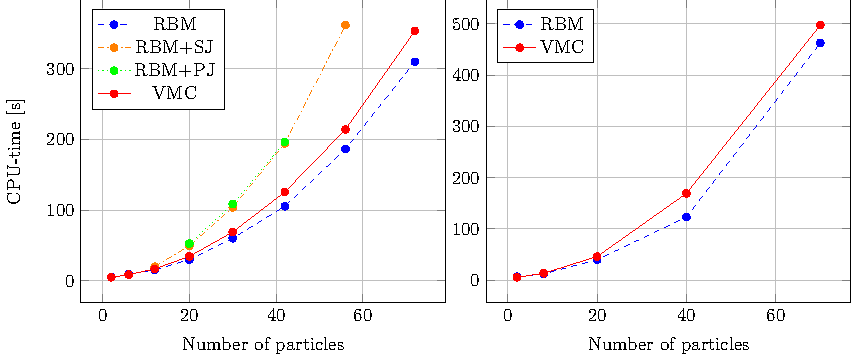
\includegraphics[scale=0.5]{figures/quantumdots.pdf}
        \caption{Speed-up obtained when
using Restricted Boltzmann machines (RBM) for systems of
two-dimensional quantum dots (with $N=2,6,12,20,30,42,56,72$
electrons) compared with a Variational Monte Carlo calculation
(VMC). The results for the energies are similar. The main speed-up is
due to a simpler mathematical form for the correlated part of the
trial wave function. In the RBM calculation we used a simple Slater
determinant for the electrons using Hermite polynomials only. However,
the results for energies and other observables can be improved upon by
multiplying the NQS with a Jastrow factor (RBM+PJ/SJ).}
\end{figure}




Applications of ML to quantum many-body problems have seen a fast-pace
progress in the past few years, touching a diverse selection of topics
ranging from numerical simulation to data analysis. The potential of
ML techniques has already surfaced in this context, already showing
improved performance with respect to existing techniques on selected
problems. To a large extent, however, the real power of ML techniques
in this domain has been only partially demonstrated, and several open
problems remain to be addressed.
In the context of variational studies with NQS, for example, the
origin of the empirical success obtained so far with different kind of
neural network quantum states is not equally well understood as for
other families of variational states, like tensor networks. Key open
challenges remain also with the representation and simulation of
fermionic systems, for which efficient neural-network representation
are still to be found.



The real challenge however is to extend these studies to nuclear
systems. Applying ML methods to nuclear systems based on the above
approaches is our central goal for the next five to ten years.  Reliable estimates of properties of infinite nuclear matter are expected to be of great importance for the experimental program at FRIB.



\subsection{Bayesian Machine Learning}

Merging a frequentist approach (the standard path in ML theory) with a Bayesian approach, has the potential to infer better probabilitity distributions and error estimates. As an example, methods for fast Monte-Carlo- based Bayesian computation of nuclear density functionals show great promise in providing a better understanding 

\subsection{Machine Learning and Quantum Computing}
Machine Learning and Quantum Computing is a very interesting avenue to explore.



\section{Education and Work force development}

AI, ML, statistical data analysis and related areas are expected to
play an ever-increasing role in many areas, from fundamental and
applied research at universities and national laboratories to
applications and developments in both the private and the public
sectors.
Developing basic research activities in these frontier
computational technologies is thus of strategic importance for our
society’s capability to address future scientific problems. Transfer
of knowledge to other disciplines and sectors, as well as developing
lasting collaborations with partners outside the traditional
university sector, are themes we expect will benefit society at large
and that will play central roles. Nuclear Physics keeps attracting many brilliant young researchers and providing our work force with these competences and skills for solving complicated physics problems is a compelling task for our community.

More text will come.

\begin{itemize}
\item In order to develop education and training efforts that target AI and ML related methods applied to Nuclear Physics, we  organized in 2019 a four day long  FRIB-TA workshop on ML methods in Nuclear physics at the NSCL/FRIB, with more than 100 participants.

\item In 2020 several of us (Bazin, Hjorth-Jensen and Liddick) will teach a three-week long Nuclear Talent course on Machine Learning and Data Analysis applied to nuclear physics. 
\end{itemize}


\section{References}


\begin{itemize}
\item An excellent reference, \href{{https://arxiv.org/abs/1803.08823}}{Mehta et al.} and \href{{https://www.sciencedirect.com/science/article/pii/S0370157319300766?via%3Dihub}}{Physics Reports (2019)}.

\item \href{{https://arxiv.org/abs/1903.10563}}{Machine Learning and the Physical Sciences by Carleo et al}

\item \href{{https://arxiv.org/pdf/1909.02487.pdf}}{Many-electron systems with Deep Learning}

\item \href{{https://journals.aps.org/prl/abstract/10.1103/PhysRevLett.120.156001}}{Every issue of Physical Review Letters has now one or more articles on ML}

\item \href{{https://github.com/copperwire/thesis/blob/master/main.pdf}}{Classifying Nuclear Physics  experiments from FRIB/NSCL}


\end{itemize}












\end{document}

